% APS360 Project Final Report (PDF)
% Compile:
%   pdflatex final_report.tex
%
% Note: This file is designed to fit the 4-page main-text limit. If you change
% figures/tables, re-check the page count after compiling.

\documentclass[10pt,twocolumn]{article}

\usepackage[margin=0.75in]{geometry}
\usepackage{times}
\usepackage{microtype}
\usepackage{amsmath}
\usepackage{amssymb}
\usepackage{booktabs}
\usepackage{graphicx}
\usepackage{siunitx}
\usepackage{enumitem}
\usepackage{xcolor}
\usepackage[hidelinks]{hyperref}
\usepackage{tikz}
\usetikzlibrary{positioning,arrows.meta}
\usepackage{pgfplots}
\usepackage{subcaption}

\pgfplotsset{compat=1.18}

\setlength{\columnsep}{0.22in}
\setlist[itemize]{leftmargin=*, nosep}
\setlist[enumerate]{leftmargin=*, nosep}
\setlength{\parindent}{0pt}

% -----------------------------
% Key numbers (from results_all.csv; full feature tensor)
% -----------------------------
\newcommand{\NTotal}{597{,}928}
\newcommand{\NTrain}{418{,}549}
\newcommand{\NVal}{89{,}689}
\newcommand{\NTest}{89{,}690}

% Best single-run (random split, full features; seed=42)
\newcommand{\AnnTestRmse}{0.1433}
\newcommand{\AnnTestAcc}{92.62}
\newcommand{\AnnParams}{629{,}340}

% Robustness (eval_suite; full features): mean ± std across seeds/splits
\newcommand{\AnnRandRmseMean}{0.1420}
\newcommand{\AnnRandRmseStd}{0.0036}
\newcommand{\AnnRandAccMean}{92.64}
\newcommand{\AnnRandAccStd}{0.31}

% Hedonic baseline robustness (eval_suite; full features)
\newcommand{\HedRandRmseMean}{0.2446}
\newcommand{\HedRandRmseStd}{0.0030}
\newcommand{\HedRandAccMean}{87.76}
\newcommand{\HedRandAccStd}{0.10}

% DeepFM robustness (3 full-train seeds: 0/1/42; full features)
\newcommand{\DeepRandRmseMean}{0.1708}
\newcommand{\DeepRandRmseStd}{0.0085}
\newcommand{\DeepRandAccMean}{91.22}
\newcommand{\DeepRandAccStd}{0.51}

% DeepFM best full-train run (random split; seed=1)
\newcommand{\DeepfmTestRmse}{0.1621}
\newcommand{\DeepfmTestAcc}{91.80}

% Hedonic baseline (random split; full features)
\newcommand{\HedTestRmse}{0.2428}
\newcommand{\HedTestAcc}{87.74}

% Additional baselines (full features; full train; seed=42)
\newcommand{\FmParams}{123{,}302}
\newcommand{\FmTestRmse}{0.2169}
\newcommand{\FmTestAcc}{89.34}
\newcommand{\FmTimeTestRmse}{0.5090}
\newcommand{\FmTimeTestAcc}{82.37}

\newcommand{\TabnetParams}{839{,}892}
\newcommand{\TabnetTestRmse}{0.3907}
\newcommand{\TabnetTestAcc}{78.11}
\newcommand{\TabnetTimeTestRmse}{0.4349}
\newcommand{\TabnetTimeTestAcc}{75.08}

% Transformer baseline (full features; train cap=50k; seed=42)
\newcommand{\FtParams}{617{,}409}
\newcommand{\FtTestRmse}{0.2138}
\newcommand{\FtTestAcc}{88.66}
\newcommand{\FtTimeTestRmse}{0.2426}
\newcommand{\FtTimeTestAcc}{86.63}

% Feature-set ablation (single run; basic feature tensor ann_tensors.pt; random split seed=42)
\newcommand{\BasicAnnTestRmse}{0.3088}
\newcommand{\BasicAnnTestAcc}{82.54}
\newcommand{\BasicHedTestRmse}{0.4722}
\newcommand{\BasicHedTestAcc}{76.42}

% Naïve constant baselines (random split; predict train mean/median log1p(price))
\newcommand{\NaiveMeanRmse}{0.5618}
\newcommand{\NaiveMeanAcc}{66.10}

% New-data proxy: time split (train earlier years, test later years; eval_suite mean ± std)
\newcommand{\AnnTimeRmseMean}{0.3146}
\newcommand{\AnnTimeRmseStd}{0.0365}
\newcommand{\AnnTimeAccMean}{82.78}
\newcommand{\AnnTimeAccStd}{2.35}
\newcommand{\HedTimeRmseMean}{0.5947}
\newcommand{\HedTimeRmseStd}{0.0162}
\newcommand{\HedTimeAccMean}{69.35}
\newcommand{\HedTimeAccStd}{1.09}
\newcommand{\DeepTimeRmseMean}{0.3533}
\newcommand{\DeepTimeRmseStd}{0.0107}
\newcommand{\DeepTimeAccMean}{75.74}
\newcommand{\DeepTimeAccStd}{1.51}

\title{House Price Prediction with Neural Tabular Models\\
\vspace{-2mm}
\large Hedonic Baseline vs Embedding+MLP ANN (APS360 Final Report)}

% TODO (submission): replace with your group member names + student numbers.
\author{RPSAps360 Group}
\date{}

\begin{document}
\maketitle

\begin{abstract}
We predict housing \texttt{TransactionPrice} from tabular transaction records using neural models that combine standardized numeric features with learned embeddings for high-cardinality categoricals. Across \NTotal cleaned transactions, our embedding+MLP ANN substantially improves over both a classic hedonic regression baseline and a DeepFM neural baseline. On \textbf{random splits} (21 robustness runs), ANN achieves \AnnRandRmseMean\(\pm\)\AnnRandRmseStd test RMSE(log) and \AnnRandAccMean\(\pm\)\AnnRandAccStd\% accuracy, vs hedonic \HedRandRmseMean\(\pm\)\HedRandRmseStd RMSE(log) and \HedRandAccMean\(\pm\)\HedRandAccStd\% accuracy. To evaluate performance on \textbf{new} samples, we use a \textbf{time-based split} (train early years \(\rightarrow\) test later years), where the ANN remains stronger: \AnnTimeRmseMean\(\pm\)\AnnTimeRmseStd RMSE(log) and \AnnTimeAccMean\(\pm\)\AnnTimeAccStd\% accuracy.
\end{abstract}

\section{Introduction (motivation + goal)}
Accurate home price estimates are useful for appraisal, market analytics, and decision support. However, price depends on nonlinear interactions between property attributes (e.g., size), location (neighborhood/city), and time (market regime). \textbf{Goal:} learn a model \(f(x)\) that predicts \(\log(1+\text{price})\) from transaction features. \textbf{Why ML:} the mapping is high-dimensional and interaction-heavy; learned embeddings and nonlinear networks can represent effects that linear models cannot, while still training efficiently on tabular data.

\begin{figure}[t]
\centering
\vspace{-1mm}
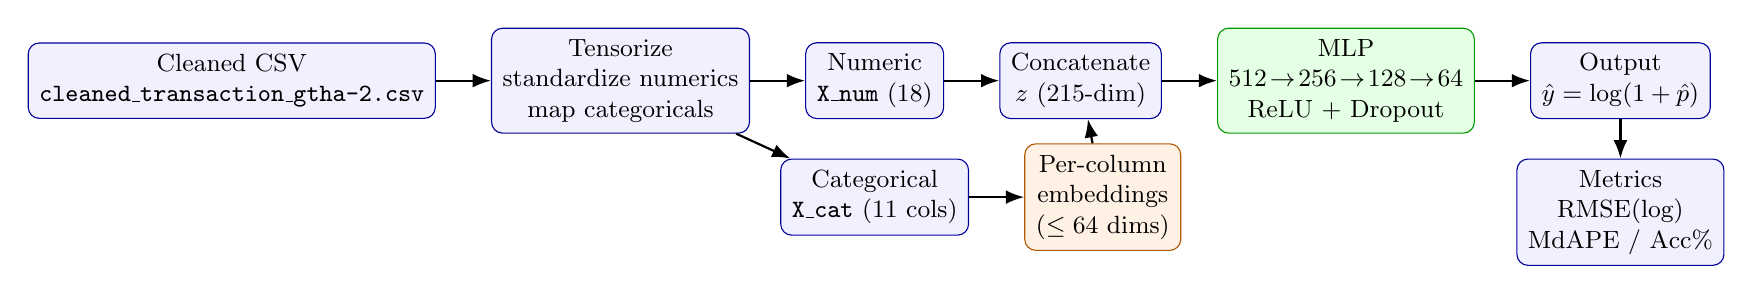
\begin{tikzpicture}[
  node/.style={draw, rounded corners, align=center, inner sep=4pt, font=\small},
  arrow/.style={-Latex, thick},
  box/.style={node, fill=blue!6, draw=blue!60!black},
  emb/.style={node, fill=orange!10, draw=orange!70!black},
  mlp/.style={node, fill=green!10, draw=green!60!black},
]
\node[box] (csv) {Cleaned CSV\\\texttt{cleaned\_transaction\_gtha-2.csv}};
\node[box, right=7mm of csv] (ten) {Tensorize\\standardize numerics\\map categoricals};
\node[box, right=7mm of ten] (num) {Numeric\\\texttt{X\_num} (18)};
\node[box, below=5mm of num] (cat) {Categorical\\\texttt{X\_cat} (11 cols)};
\node[emb, right=7mm of cat] (embs) {Per-column\\embeddings\\(\(\le 64\) dims)};
\node[box, right=7mm of num] (concat) {Concatenate\\\(z\) (215-dim)};
\node[mlp, right=7mm of concat] (mlp) {MLP\\\(512\!\rightarrow\!256\!\rightarrow\!128\!\rightarrow\!64\)\\ReLU + Dropout};
\node[box, right=7mm of mlp] (out) {Output\\\(\hat{y}=\log(1+\hat{p})\)};
\node[box, below=5mm of out] (met) {Metrics\\RMSE(log)\\MdAPE / Acc\%};
\draw[arrow] (csv) -- (ten);
\draw[arrow] (ten) -- (num);
\draw[arrow] (ten) -- (cat);
\draw[arrow] (num) -- (concat);
\draw[arrow] (cat) -- (embs);
\draw[arrow] (embs) -- (concat);
\draw[arrow] (concat) -- (mlp);
\draw[arrow] (mlp) -- (out);
\draw[arrow] (out) -- (met);
\end{tikzpicture}
\vspace{-2mm}
\caption{Illustration: the core idea is to represent high-cardinality categoricals via embeddings, concatenate with numeric features, and train an MLP to predict \(\log(1+\text{price})\).}
\label{fig:pipeline}
\end{figure}

\section{Background \& related work (5+)}
\begin{itemize}
  \item \textbf{Hedonic regression} models price as a sum of attribute effects and is a standard baseline in housing economics (\cite{rosen1974hedonic}).
  \item \textbf{Factorization Machines (FM)} represent pairwise feature interactions with low-rank factors, often effective for sparse/high-cardinality settings (\cite{rendle2010fm}).
  \item \textbf{DeepFM} combines linear terms, FM interactions, and a deep MLP to capture both low- and high-order effects in tabular data (\cite{guo2017deepfm}).
  \item \textbf{TabNet} uses attentive feature selection and sparse masks as an alternative inductive bias for tabular learning (\cite{arik2019tabnet}).
  \item \textbf{FT-Transformer} tokenizes features and applies Transformer self-attention for tabular prediction (\cite{gorishniy2021revisiting}).
  \item \textbf{Gradient-boosted trees} (XGBoost/LightGBM) are widely used strong baselines for tabular regression/classification (\cite{chen2016xgboost,ke2017lightgbm}).
\end{itemize}

\section{Data processing (sources, steps, stats)}
\textbf{Source.} The dataset is a cleaned snapshot of Greater Toronto and Hamilton Area (GTHA) housing transactions derived from the RPS proposal pipeline (appraisal-form extracts + transaction feeds) and stored as \texttt{cleaned\_transaction\_gtha-2.csv}.

\textbf{Tensorization.} We run \texttt{prepare\_ann\_tensors.py} to create a single \texttt{.pt} file containing:
(i) standardized numeric tensor \(X_{\text{num}}\),
(ii) categorical index tensor \(X_{\text{cat}}\) (for embedding lookups),
(iii) targets \(y=\text{price}\) and \(y_{\log}=\log(1+y)\),
plus metadata (column lists, category maps, mean/std).

\textbf{Cleaning.} We drop invalid targets (missing/non-positive price), standardize numeric columns with streaming mean/std (Welford), impute missing numeric values to the mean (standardized value becomes 0), map missing categoricals to \texttt{\_\_NA\_\_}, and optionally cap rare categories to \texttt{\_\_OTHER\_\_}.

\textbf{Features.} We report results on the \texttt{full} feature set: 18 numeric (e.g., \texttt{LivingArea, LotSize, YearBuilt, gcode\_Lat, gcode\_Lon, TransactionYear, Quarter, DOM}) and 11 categorical (e.g., \texttt{BuildingType, PropertyStyle, FSA, gcode\_City, Basement, Ownership, PropertyUse}); see \texttt{prepare\_ann\_tensors.py} for the complete lists.

\textbf{Basic statistics.} \NTotal transactions; random split produces \NTrain/\NVal/\NTest train/val/test rows. Raw prices range from \(\$10{,}000\) to \(\$22{,}000{,}000\) (median \(\$570{,}000\)). High-cardinality categoricals motivate embeddings (e.g., \texttt{PropertyStyle}: 3{,}356; \texttt{PropertyUse}: 2{,}284; \texttt{BuildingType}: 995). Example cleaned row: \texttt{LivingArea=2160}, \texttt{YearBuilt=1989}, \texttt{FSA=L0H}, \texttt{TransactionYear=2009}, \texttt{price=600000}.

\begin{figure}[t]
\centering
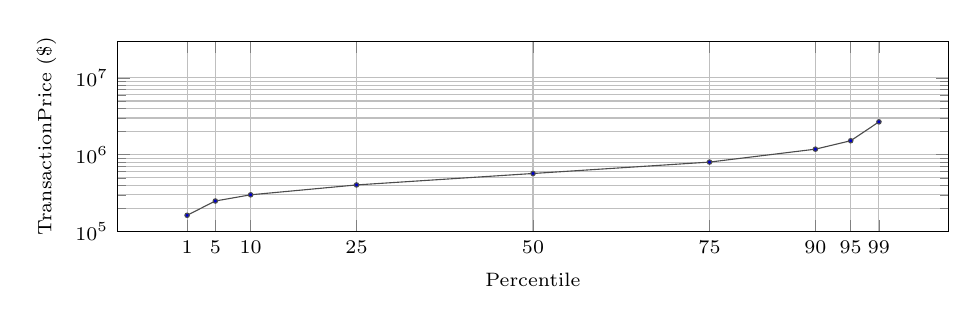
\begin{tikzpicture}
\begin{axis}[
  width=\columnwidth,
  height=4.0cm,
  xlabel={Percentile},
  ylabel={TransactionPrice (\$)},
  ymode=log,
  log basis y=10,
  ymin=1e5, ymax=3e7,
  xtick={1,5,10,25,50,75,90,95,99},
  grid=both,
  tick label style={font=\scriptsize},
  label style={font=\scriptsize},
]
\addplot+[mark=*, mark size=0.8pt, color=black!70] coordinates {
  (1,163000)
  (5,250000)
  (10,301000)
  (25,404486)
  (50,570000)
  (75,801800)
  (90,1181000)
  (95,1520000)
  (99,2675365)
};
\end{axis}
\end{tikzpicture}
\vspace{-2mm}
\caption{Price distribution in the cleaned dataset (log y-axis). Points are selected percentiles of \texttt{TransactionPrice}.}
\label{fig:price-dist}
\end{figure}

\section{Models}
\subsection{Baseline: hedonic regression (fixed effects)}
We implement a linear baseline:
\[
  \hat{y}=b+w^\top x_{\text{num}} + \sum_j \beta^{(j)}[x_{\text{cat},j}],
\]
where each categorical column \(j\) has a learned per-category coefficient \(\beta^{(j)}\). This is equivalent to one-hot regression, implemented efficiently via 1D embedding tables. We train it on the same split/metrics as the ANN and select the best checkpoint by validation MSE for fair comparison.
For our robustness evaluation, we use batch size 8192, \(lr=0.01\), 20 epochs, and no weight decay.

\subsection{Primary model: embedding+MLP ANN (architecture)}
For high-cardinality categoricals (e.g., city/style), one-hot is impractical, so we learn embeddings and concatenate them with numeric features:
\[
  z = [x_{\text{num}}, \text{Emb}_1(x_{\text{cat},1}), \dots, \text{Emb}_J(x_{\text{cat},J})],\quad
  \hat{y}=\text{MLP}(z).
\]
\textbf{Best config (full features):} hidden sizes \(512\rightarrow256\rightarrow128\rightarrow64\), dropout \(0.1\), embedding cap \(64\), AdamW \(lr=0.004\), weight decay \(0.001\), batch size 512, 30 epochs with checkpoint selection by validation MSE (best epoch 28 for seed=42). Embedding dimensions use a \(\sqrt{|V|}\) rule capped at 64, resulting in a 215-dim concatenated input. Parameter count \(\approx\)\AnnParams; a reference run (seed=42) achieves \AnnTestRmse test RMSE(log) and \AnnTestAcc\% accuracy.

\subsection{Additional neural baseline: DeepFM}
DeepFM combines (i) linear terms, (ii) low-rank pairwise interactions (FM), and (iii) a deep MLP over numeric features plus categorical factor embeddings. Our best DeepFM uses factor dimension \(k=16\), hidden sizes \(2048\rightarrow1024\rightarrow512\), dropout 0.05, AdamW \(lr=0.002\), weight decay \(0.001\), batch size 4096, and 40 epochs (checkpoint by validation MSE).

\subsection{Additional baselines: FM, TabNet, FT-Transformer}
\textbf{FM} models all pairwise feature interactions via low-rank factors, often strong for sparse/high-cardinality problems. \textbf{TabNet} uses sequential attentive feature selection with sparse masks. \textbf{FT-Transformer} tokenizes each feature into a vector and applies self-attention to learn cross-feature interactions.

\section{Evaluation protocol and metrics}
\textbf{Train/val/test splits.} We use (i) a standard 70/15/15 random split and report robustness by repeating over multiple model seeds and split seeds, and (ii) a time-based split that sorts by (\texttt{TransactionYear}, \texttt{Quarter}) and partitions 70/15/15 by time order (with a seeded random tiebreak within the same year/quarter). We tune using validation only and treat the test split as a one-time evaluation.

\textbf{Metrics.} We train on log-space MSE and report RMSE(log). For interpretability, we also report MdAPE in price space and a derived accuracy:
\(\mathrm{Acc}\%=\max(0,100(1-\mathrm{MdAPE}))\).

\section{Quantitative results}
\textbf{Sanity-check floor.} A constant predictor (train-mean \(\log(1+\text{price})\)) achieves \NaiveMeanRmse test RMSE(log) and \NaiveMeanAcc\% accuracy on the random split, confirming the task is non-trivial.

\begin{table*}[t]
\centering
\scriptsize
\setlength{\tabcolsep}{4pt}
\begin{tabular}{@{}lrrrrr@{}}
\toprule
Model & Params & Rand RMSE(log) & Rand Acc(\%) & Time RMSE(log) & Time Acc(\%) \\
\midrule
Constant (mean) & 0 & \NaiveMeanRmse & \NaiveMeanAcc & -- & -- \\
Hedonic & 7{,}254 & \HedRandRmseMean\(\pm\)\HedRandRmseStd & \HedRandAccMean\(\pm\)\HedRandAccStd & \HedTimeRmseMean\(\pm\)\HedTimeRmseStd & \HedTimeAccMean\(\pm\)\HedTimeAccStd \\
FM (2-way) & \FmParams & \FmTestRmse & \FmTestAcc & \FmTimeTestRmse & \FmTimeTestAcc \\
TabNet & \TabnetParams & \TabnetTestRmse & \TabnetTestAcc & \TabnetTimeTestRmse & \TabnetTimeTestAcc \\
FT-Transformer & \FtParams & \FtTestRmse & \FtTestAcc & \FtTimeTestRmse & \FtTimeTestAcc \\
DeepFM & 3{,}146{,}151 & \DeepRandRmseMean\(\pm\)\DeepRandRmseStd & \DeepRandAccMean\(\pm\)\DeepRandAccStd & \DeepTimeRmseMean\(\pm\)\DeepTimeRmseStd & \DeepTimeAccMean\(\pm\)\DeepTimeAccStd \\
ANN (embed+MLP) & \AnnParams & \AnnRandRmseMean\(\pm\)\AnnRandRmseStd & \AnnRandAccMean\(\pm\)\AnnRandAccStd & \AnnTimeRmseMean\(\pm\)\AnnTimeRmseStd & \AnnTimeAccMean\(\pm\)\AnnTimeAccStd \\
\bottomrule
\end{tabular}
\vspace{-2mm}
\caption{Performance summary on the full feature set. ANN/Hedonic are averaged over robustness runs (random: 21; time: 9). DeepFM is averaged over 3 full-train seeds (0/1/42). FM and TabNet are single full-train runs (seed=42). FT-Transformer is a single run (seed=42) trained with a 50k train cap for CPU feasibility.}
\label{tab:all-models}
\end{table*}

\begin{figure*}[t]
\centering
\begin{subfigure}{0.49\linewidth}
\centering
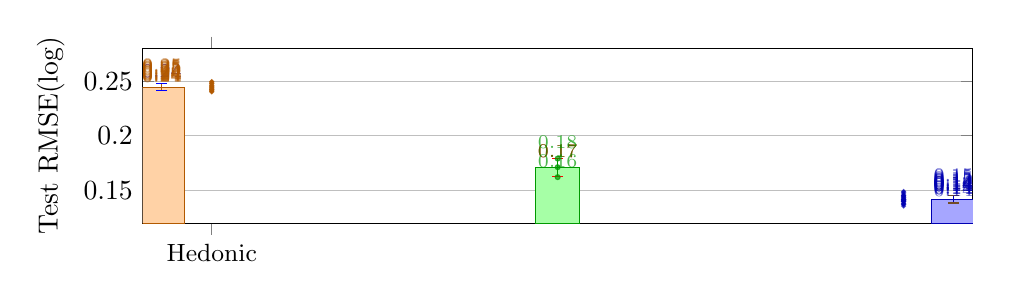
\begin{tikzpicture}
\begin{axis}[
  ybar,
  width=\linewidth,
  height=3.8cm,
  bar width=16pt,
  ylabel={Test RMSE(log)},
  symbolic x coords={Hedonic,DeepFM,ANN},
  xtick=data,
  ymin=0.12, ymax=0.28,
  ymajorgrids=true,
  error bars/y dir=both,
  error bars/y explicit,
  nodes near coords,
  every node near coord/.append style={font=\scriptsize},
  xticklabel style={font=\small},
]
\addplot+[fill=orange!35, draw=orange!70!black] coordinates {(Hedonic,\HedRandRmseMean) +- (0,\HedRandRmseStd)};
\addplot+[fill=green!35, draw=green!60!black] coordinates {(DeepFM,\DeepRandRmseMean) +- (0,\DeepRandRmseStd)};
\addplot+[fill=blue!35, draw=blue!70!black] coordinates {(ANN,\AnnRandRmseMean) +- (0,\AnnRandRmseStd)};
\addplot+[only marks, mark=*, mark size=0.7pt, color=orange!70!black, opacity=0.6] coordinates {
  (Hedonic,0.2426) (Hedonic,0.2402) (Hedonic,0.2497) (Hedonic,0.2480) (Hedonic,0.2476) (Hedonic,0.2439) (Hedonic,0.2424) (Hedonic,0.2408) (Hedonic,0.2422) (Hedonic,0.2494) (Hedonic,0.2475) (Hedonic,0.2491) (Hedonic,0.2459) (Hedonic,0.2441) (Hedonic,0.2459) (Hedonic,0.2452) (Hedonic,0.2431) (Hedonic,0.2447) (Hedonic,0.2419) (Hedonic,0.2405) (Hedonic,0.2416)
};
\addplot+[only marks, mark=*, mark size=0.9pt, color=green!60!black, opacity=0.7] coordinates {
  (DeepFM,0.1791) (DeepFM,0.1712) (DeepFM,0.1621)
};
\addplot+[only marks, mark=*, mark size=0.7pt, color=blue!70!black, opacity=0.6] coordinates {
  (ANN,0.1434) (ANN,0.1399) (ANN,0.1375) (ANN,0.1466) (ANN,0.1370) (ANN,0.1409) (ANN,0.1447) (ANN,0.1452) (ANN,0.1480) (ANN,0.1438) (ANN,0.1356) (ANN,0.1409) (ANN,0.1490) (ANN,0.1396) (ANN,0.1418) (ANN,0.1397) (ANN,0.1380) (ANN,0.1426) (ANN,0.1416) (ANN,0.1414) (ANN,0.1450)
};
\end{axis}
\end{tikzpicture}
\caption{Random split RMSE (mean \(\pm\) std; ANN/Hedonic \(n=21\), DeepFM \(n=3\)).}
\end{subfigure}
\hfill
\begin{subfigure}{0.49\linewidth}
\centering
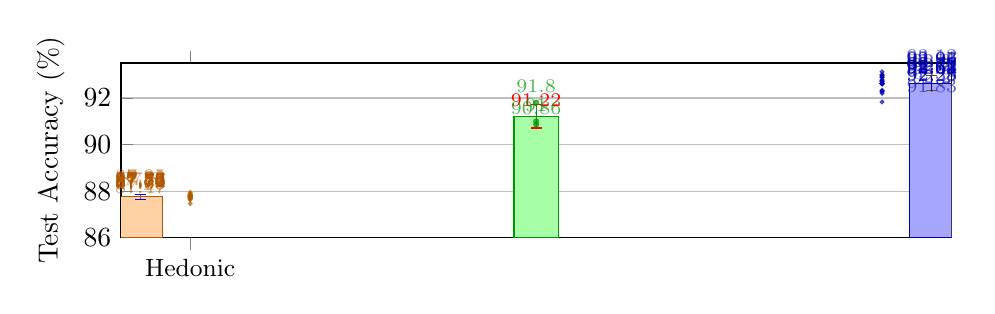
\begin{tikzpicture}
\begin{axis}[
  ybar,
  width=\linewidth,
  height=3.8cm,
  bar width=16pt,
  ylabel={Test Accuracy (\%)},
  symbolic x coords={Hedonic,DeepFM,ANN},
  xtick=data,
  ymin=86, ymax=93.5,
  ymajorgrids=true,
  error bars/y dir=both,
  error bars/y explicit,
  nodes near coords,
  every node near coord/.append style={font=\scriptsize},
  xticklabel style={font=\small},
]
\addplot+[fill=orange!35, draw=orange!70!black] coordinates {(Hedonic,\HedRandAccMean) +- (0,\HedRandAccStd)};
\addplot+[fill=green!35, draw=green!60!black] coordinates {(DeepFM,\DeepRandAccMean) +- (0,\DeepRandAccStd)};
\addplot+[fill=blue!35, draw=blue!70!black] coordinates {(ANN,\AnnRandAccMean) +- (0,\AnnRandAccStd)};
\addplot+[only marks, mark=*, mark size=0.7pt, color=orange!70!black, opacity=0.6] coordinates {
  (Hedonic,87.7199) (Hedonic,87.9470) (Hedonic,87.8302) (Hedonic,87.8754) (Hedonic,87.4666) (Hedonic,87.6624) (Hedonic,87.7216) (Hedonic,87.7659) (Hedonic,87.7390) (Hedonic,87.7773) (Hedonic,87.8040) (Hedonic,87.7355) (Hedonic,87.7418) (Hedonic,87.8550) (Hedonic,87.6301) (Hedonic,87.7703) (Hedonic,87.8154) (Hedonic,87.7429) (Hedonic,87.8378) (Hedonic,87.6905) (Hedonic,87.8113)
};
\addplot+[only marks, mark=*, mark size=0.9pt, color=green!60!black, opacity=0.7] coordinates {
  (DeepFM,90.9951) (DeepFM,90.8615) (DeepFM,91.8002)
};
\addplot+[only marks, mark=*, mark size=0.7pt, color=blue!70!black, opacity=0.6] coordinates {
  (ANN,92.7739) (ANN,92.9570) (ANN,93.0117) (ANN,92.2799) (ANN,92.9697) (ANN,92.6272) (ANN,92.7600) (ANN,92.6082) (ANN,92.3316) (ANN,92.2886) (ANN,92.8901) (ANN,92.6005) (ANN,91.8307) (ANN,92.7244) (ANN,92.6367) (ANN,92.8954) (ANN,93.1237) (ANN,92.6203) (ANN,92.6233) (ANN,92.7038) (ANN,92.2001)
};
\end{axis}
\end{tikzpicture}
\caption{Random split accuracy (mean \(\pm\) std; ANN/Hedonic \(n=21\), DeepFM \(n=3\)).}
\end{subfigure}

\vspace{0.5mm}

\begin{subfigure}{0.49\linewidth}
\centering
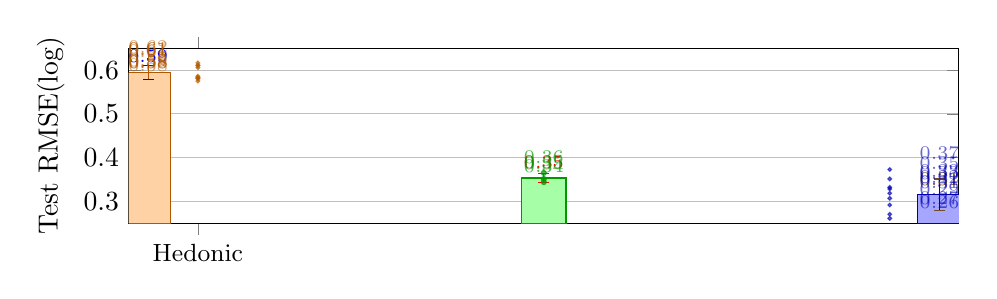
\begin{tikzpicture}
\begin{axis}[
  ybar,
  width=\linewidth,
  height=3.8cm,
  bar width=16pt,
  ylabel={Test RMSE(log)},
  symbolic x coords={Hedonic,DeepFM,ANN},
  xtick=data,
  ymin=0.25, ymax=0.65,
  ymajorgrids=true,
  error bars/y dir=both,
  error bars/y explicit,
  nodes near coords,
  every node near coord/.append style={font=\scriptsize},
  xticklabel style={font=\small},
]
\addplot+[fill=orange!35, draw=orange!70!black] coordinates {(Hedonic,\HedTimeRmseMean) +- (0,\HedTimeRmseStd)};
\addplot+[fill=green!35, draw=green!60!black] coordinates {(DeepFM,\DeepTimeRmseMean) +- (0,\DeepTimeRmseStd)};
\addplot+[fill=blue!35, draw=blue!70!black] coordinates {(ANN,\AnnTimeRmseMean) +- (0,\AnnTimeRmseStd)};
\addplot+[only marks, mark=*, mark size=0.7pt, color=orange!70!black, opacity=0.6] coordinates {
  (Hedonic,0.6106) (Hedonic,0.5808) (Hedonic,0.6059) (Hedonic,0.5864) (Hedonic,0.6114) (Hedonic,0.5815) (Hedonic,0.6168) (Hedonic,0.5752) (Hedonic,0.5833)
};
\addplot+[only marks, mark=*, mark size=0.9pt, color=green!60!black, opacity=0.7] coordinates {
  (DeepFM,0.3438) (DeepFM,0.3511) (DeepFM,0.3649)
};
\addplot+[only marks, mark=*, mark size=0.7pt, color=blue!70!black, opacity=0.6] coordinates {
  (ANN,0.3319) (ANN,0.3511) (ANN,0.3727) (ANN,0.3068) (ANN,0.2915) (ANN,0.2609) (ANN,0.3281) (ANN,0.3183) (ANN,0.2703)
};
\end{axis}
\end{tikzpicture}
\caption{Time split RMSE (mean \(\pm\) std; ANN/Hedonic \(n=9\), DeepFM \(n=3\)).}
\end{subfigure}
\hfill
\begin{subfigure}{0.49\linewidth}
\centering
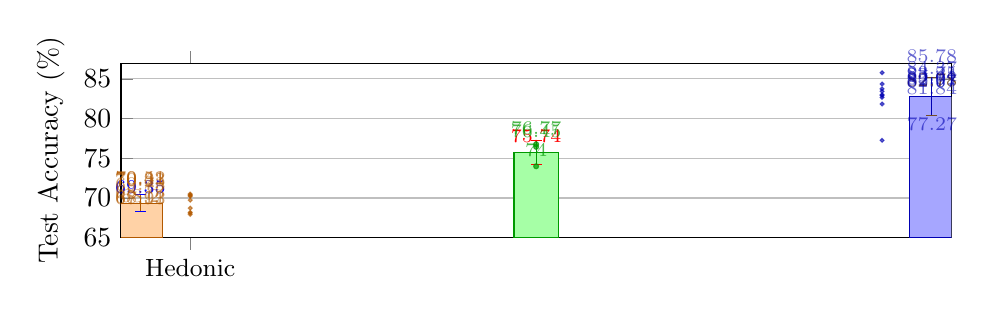
\begin{tikzpicture}
\begin{axis}[
  ybar,
  width=\linewidth,
  height=3.8cm,
  bar width=16pt,
  ylabel={Test Accuracy (\%)},
  symbolic x coords={Hedonic,DeepFM,ANN},
  xtick=data,
  ymin=65, ymax=87,
  ymajorgrids=true,
  error bars/y dir=both,
  error bars/y explicit,
  nodes near coords,
  every node near coord/.append style={font=\scriptsize},
  xticklabel style={font=\small},
]
\addplot+[fill=orange!35, draw=orange!70!black] coordinates {(Hedonic,\HedTimeAccMean) +- (0,\HedTimeAccStd)};
\addplot+[fill=green!35, draw=green!60!black] coordinates {(DeepFM,\DeepTimeAccMean) +- (0,\DeepTimeAccStd)};
\addplot+[fill=blue!35, draw=blue!70!black] coordinates {(ANN,\AnnTimeAccMean) +- (0,\AnnTimeAccStd)};
\addplot+[only marks, mark=*, mark size=0.7pt, color=orange!70!black, opacity=0.6] coordinates {
  (Hedonic,68.2017) (Hedonic,70.2305) (Hedonic,68.7268) (Hedonic,69.7324) (Hedonic,68.1137) (Hedonic,70.5108) (Hedonic,67.9282) (Hedonic,70.4157) (Hedonic,70.3063)
};
\addplot+[only marks, mark=*, mark size=0.9pt, color=green!60!black, opacity=0.7] coordinates {
  (DeepFM,76.4491) (DeepFM,76.7739) (DeepFM,74.0039)
};
\addplot+[only marks, mark=*, mark size=0.7pt, color=blue!70!black, opacity=0.6] coordinates {
  (ANN,81.8443) (ANN,82.9056) (ANN,77.2688) (ANN,83.0138) (ANN,83.7456) (ANN,85.7801) (ANN,82.6667) (ANN,83.4415) (ANN,84.3658)
};
\end{axis}
\end{tikzpicture}
\caption{Time split accuracy (mean \(\pm\) std; ANN/Hedonic \(n=9\), DeepFM \(n=3\)).}
\end{subfigure}

\vspace{-1mm}
\caption{Quantitative results on the full feature set with error bars. Random split: ANN/Hedonic are averaged over 21 robustness runs; DeepFM is averaged over 3 full-train seeds (0/1/42). Time split: ANN/Hedonic are averaged over 9 robustness runs; DeepFM is averaged over 3 full-train seeds.}
\label{fig:results}
\end{figure*}

\section{Qualitative results (sample predictions)}
To contextualize quantitative error, we show three test examples chosen by absolute percentage error (APE) percentiles (5th/50th/95th). This highlights both typical behavior and failure modes.
\begin{table}[t]
\centering
\small
\begin{tabular}{@{}lrrr@{}}
\toprule
Example & True (\$) & Pred (\$) & APE (\%) \\
\midrule
p5 (very accurate) & 1{,}020{,}000 & 1{,}026{,}681 & 0.66 \\
p50 (typical) & 797{,}900 & 738{,}979 & 7.38 \\
p95 (large error) & 260{,}000 & 334{,}129 & 28.51 \\
\bottomrule
\end{tabular}
\vspace{-2mm}
\caption{Representative ANN outputs on the random-split test set. Large errors tend to occur for rare/outlier properties or distribution shifts.}
\label{tab:qual}
\end{table}

\section{Evaluation on new data (time-based split)}
\begin{figure}[t]
\centering
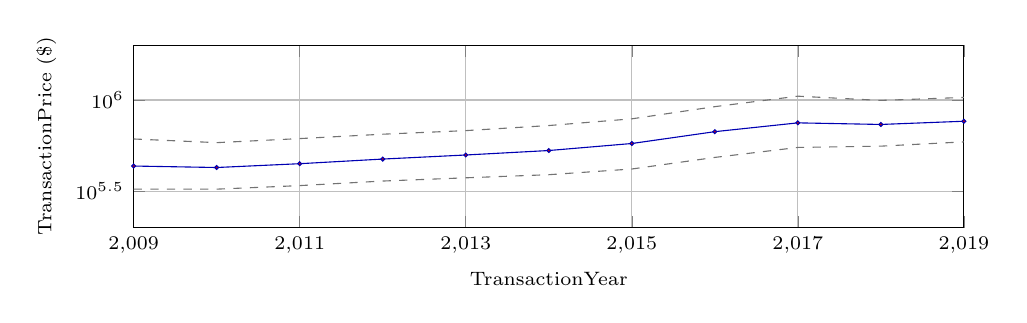
\begin{tikzpicture}
\begin{axis}[
  width=\columnwidth,
  height=3.9cm,
  xlabel={TransactionYear},
  ylabel={TransactionPrice (\$)},
  ymode=log,
  log basis y=10,
  xmin=2009, xmax=2019,
  xtick={2009,2011,2013,2015,2017,2019},
  ymin=2e5, ymax=2e6,
  grid=both,
  tick label style={font=\scriptsize},
  label style={font=\scriptsize},
]
\addplot+[mark=none, dashed, color=black!55] coordinates {
  (2009,325000) (2010,325000) (2011,339900) (2012,360000) (2013,375000) (2014,390000) (2015,419000) (2016,485000) (2017,550000) (2018,559000) (2019,590000)
};
\addplot+[mark=*, mark size=0.7pt, color=blue!70!black] coordinates {
  (2009,435000) (2010,427000) (2011,448000) (2012,475000) (2013,500000) (2014,529000) (2015,578000) (2016,671100) (2017,750000) (2018,735000) (2019,765500)
};
\addplot+[mark=none, dashed, color=black!55] coordinates {
  (2009,612000) (2010,584300) (2011,615000) (2012,650000) (2013,680000) (2014,725000) (2015,789000) (2016,920000) (2017,1050000) (2018,995000) (2019,1033625)
};
\end{axis}
\end{tikzpicture}
\vspace{-2mm}
\caption{Dataset non-stationarity (2009--2019): 25th/50th/75th price percentiles by year. Median price rises sharply, motivating time-based evaluation.}
\label{fig:market-drift}
\end{figure}

We evaluate generalization to \emph{new} samples via a time split: we order transactions by (\texttt{TransactionYear}, \texttt{Quarter}) and split 70/15/15 by time (train early \(\rightarrow\) test late), so the test set is chronologically ``future'' relative to training. With our time-split procedure (fixed \texttt{split\_seed}), train ends at \textbf{2016Q2}, validation ends at \textbf{2017Q4}, and the test set is mostly \textbf{2018--2019} transactions (Figure~\ref{fig:market-drift}). We keep model hyperparameters fixed (chosen via validation) and do not tune on the time-test labels. To reduce the chance of reporting a lucky initialization, we repeat runs across multiple seeds and report mean \(\pm\) std. Figure~\ref{fig:results} (bottom row) shows that although all models degrade under distribution shift, the ANN retains a large advantage over the hedonic baseline.

\section{Discussion (what we learned)}
\begin{figure}[t]
\centering
\begin{subfigure}{\columnwidth}
\centering
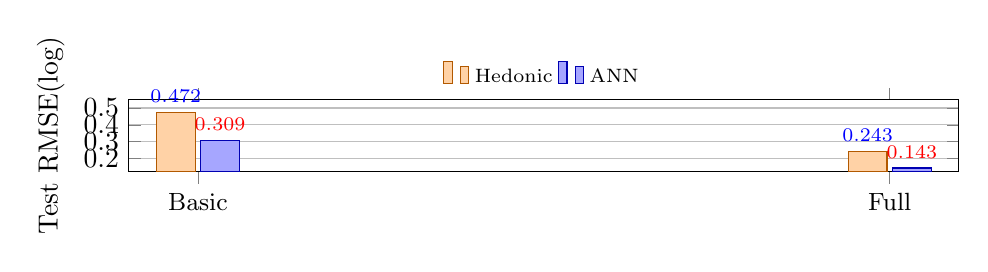
\begin{tikzpicture}
\begin{axis}[
  ybar,
  width=\linewidth,
  height=2.5cm,
  bar width=14pt,
  ylabel={Test RMSE(log)},
  symbolic x coords={Basic,Full},
  xtick=data,
  ymin=0.12, ymax=0.55,
  ymajorgrids=true,
  nodes near coords,
  nodes near coords style={/pgf/number format/fixed, /pgf/number format/precision=3},
  every node near coord/.append style={font=\scriptsize},
  xticklabel style={font=\small},
  legend style={font=\scriptsize, at={(0.5,1.02)}, anchor=south, legend columns=2, draw=none},
]
\addplot+[fill=orange!35, draw=orange!70!black] coordinates {(Basic,\BasicHedTestRmse) (Full,\HedTestRmse)};
\addplot+[fill=blue!35, draw=blue!70!black] coordinates {(Basic,\BasicAnnTestRmse) (Full,\AnnTestRmse)};
\legend{Hedonic,ANN}
\end{axis}
\end{tikzpicture}
\vspace{-2mm}
\caption{Feature-set ablation (seed=42): \texttt{basic} uses attributes only; \texttt{full} adds location+time.}
\label{fig:ablation}
\end{subfigure}

\vspace{-1mm}

\begin{subfigure}{\columnwidth}
\centering
\begin{tikzpicture}
\begin{axis}[
  xbar,
  width=\linewidth,
  height=3.3cm,
  xlabel={Increase in validation MSE (Δval MSE)},
  ytick=data,
  y dir=reverse,
  yticklabels={
    LivingArea,
    TransactionYear,
    FSA,
    gcode\_City,
    YearBuilt,
    BuildingType,
    Ownership,
    PropertyStyle
  },
  xmin=0, xmax=0.11,
  grid=both,
  tick label style={font=\scriptsize},
  label style={font=\scriptsize},
]
\addplot+[fill=blue!25, draw=blue!60!black] coordinates {
  (0.098610,0)
  (0.089895,1)
  (0.066793,2)
  (0.042350,3)
  (0.011641,4)
  (0.009254,5)
  (0.007690,6)
  (0.006414,7)
};
\end{axis}
\end{tikzpicture}
\vspace{-2mm}
\caption{Permutation importance on a random-split validation subset (20k rows; split\_seed=42).}
\label{fig:feature-importance}
\end{subfigure}

\vspace{-2mm}
\caption{Analysis: richer features yield large gains (top), and size, time, and location dominate ANN predictions (bottom).}
\label{fig:analysis}
\end{figure}

\begin{itemize}
  \item \textbf{Feature set drives performance.} Feature richness is critical: moving from \texttt{basic} (attributes only) to \texttt{full} (adds location+time) cuts ANN test RMSE(log) from \BasicAnnTestRmse\(\rightarrow\)\AnnTestRmse and raises accuracy from \BasicAnnTestAcc\(\rightarrow\)\AnnTestAcc\% (Figure~\ref{fig:ablation}); hedonic regression also improves (\BasicHedTestRmse\(\rightarrow\)\HedTestRmse).
  \item \textbf{What the model uses.} Permutation importance (Figure~\ref{fig:feature-importance}) shows that size (\texttt{LivingArea}), market trend (\texttt{TransactionYear}), and location (\texttt{FSA}/\texttt{gcode\_City}) are dominant drivers, matching domain intuition.
  \item \textbf{ANN vs baselines.} FM improves over hedonic regression by adding pairwise interactions, but the ANN (and DeepFM) is strongest overall (Table~\ref{tab:all-models}), suggesting nonlinear embeddings + deeper interaction modeling matter. TabNet underperforms in our setting, highlighting sensitivity to optimization/hyperparameters for this dataset.
  \item \textbf{New-data behavior.} Time splits are harder due to distribution shift; the ANN remains meaningfully better than hedonic regression, suggesting the improvement is not only due to random mixing across years.
  \item \textbf{Failure modes.} Large errors are concentrated in rare/outlier properties and in shifted market segments; these motivate stricter time-aware evaluation and out-of-distribution monitoring for deployment.
\end{itemize}

\section{Ethical considerations}
Housing prices encode socioeconomic inequities; a model can reproduce or amplify them if used for lending, insurance, or neighborhood ``risk'' scoring. Privacy also matters: we avoid address-level identifiers and recommend strict access controls, drift monitoring, and transparent limitations (e.g., out-of-distribution detection) for any real use.

\section{Project difficulty / quality}
This project is challenging due to the dataset scale (\(\sim\)600k rows), heavy-tailed targets, missingness, distribution shift across time, and high-cardinality categoricals. Beyond a single model, we implemented multiple baselines (hedonic regression, FM, DeepFM, TabNet, FT-Transformer), consolidated results into a single experiment log, and evaluated robustness across multiple seeds and both random and time splits. The final ANN performs better than expected for this setting while remaining feasible to train (\(\approx\)\AnnParams parameters).

\begin{thebibliography}{9}
\bibitem{rosen1974hedonic}
Sherwin Rosen.
\newblock Hedonic Prices and Implicit Markets: Product Differentiation in Pure Competition.
\newblock \emph{Journal of Political Economy}, 82(1):34--55, 1974.

\bibitem{rendle2010fm}
Steffen Rendle.
\newblock Factorization Machines.
\newblock In \emph{ICDM}, 2010.

\bibitem{guo2017deepfm}
Huifeng Guo, Ruiming Tang, Yunming Ye, Zhenguo Li, Xiuqiang He.
\newblock DeepFM: A Factorization-Machine based Neural Network for CTR Prediction.
\newblock In \emph{IJCAI}, 2017.

\bibitem{arik2019tabnet}
Sercan O. Arik, Tomas Pfister.
\newblock TabNet: Attentive Interpretable Tabular Learning.
\newblock \emph{arXiv:1908.07442}, 2019.

\bibitem{gorishniy2021revisiting}
Yury Gorishniy, Ivan Rubachev, Valentin Khrulkov, Artem Babenko.
\newblock Revisiting Deep Learning Models for Tabular Data.
\newblock In \emph{NeurIPS}, 2021.

\bibitem{chen2016xgboost}
Tianqi Chen, Carlos Guestrin.
\newblock XGBoost: A Scalable Tree Boosting System.
\newblock In \emph{KDD}, 2016.

\bibitem{ke2017lightgbm}
Guolin Ke et al.
\newblock LightGBM: A Highly Efficient Gradient Boosting Decision Tree.
\newblock In \emph{NeurIPS}, 2017.
\end{thebibliography}

\end{document}
